\chapter{基于属性保持的零样本物体分类方法}



\section{问题描述}


零样本物体识别(Zero-Shot Recogintion, ZSR)或零样本学习(Zero-Shot Learning, ZSL)是为了能够对训练过程未见过的新类别图像进行分类识别。目前,关于零样本学习问题的难点,学界的共识是如何将已见类别的知识迁移到未见类别上。尽管到目前为止,已经有非常多的零样本分类方法,这些方法都是依据一些非常简单和直观的机制。例如,虽然“浣熊”这个类别在训练的时候没有见过,但是我们仍然可以识别出浣熊的图像,通过检查浣熊这个类别特有的一些属性特征,像“有条纹的尾巴”~\cite{farhadi2009describing,lampert2009learning,zhang2013attribute,li2010object}、“像狐狸的外观”~\cite{torresani2010efficient,li2010object}、以及“浣熊”这个类别的语义信息~\cite{pennington2014glove,mikolov2013distributed}。这些属性特征通常在训练阶段被建模,然后期待在测试阶段中可以在所有的类别(已见类别和未见类别)中共享。经过数十年的发展,目前的零样本学习框架已经从初始基于属性分类器的模型~\cite{lampert2009learning}发展到基于嵌入映射的模型~\cite{akata2015label,frome2013devise,weston2010large}。这种基于嵌入映射的模型往往简单有效,如图~\ref{ch3:fig:zsl_paradigms}(a)所示,这种模型首先将图像从视觉空间(V)映射到语义空间(S),同时,图像类别的语义特征也在该语义空间中。这样映射之后,零样本学习问题就“退化”成一个最近邻的类别查找问题。

\begin{wrapfigure}{r}{0.6\linewidth}
    \centering
        \includegraphics[width=0.95\linewidth]{chapter3/res/zsl_paradigms.pdf}
    \captionof{figure}{三种典型的零样本学习框架。}
    \label{ch3:fig:zsl_paradigms}
\end{wrapfigure}

这种嵌入映射模型的知识迁移能力受限于\textbf{语义损失}的问题。如图~\ref{ch3:fig:zsl_paradigms}所示,模型丢失一些对训练集图像方差较小的属性(即,不同类之间区别小的属性)有利于训练集的分类。然而,由于训练集和测试集之间存在差异,这些“丢失”的属性可能对测试集来说具有较大的区别性,这样就会造成对测试集分类的困难。虽然类别在语义空间是一个单独的“点”,具有丰富的语义信息,但是将所有同类的图像从视觉空间映射到这个点附近,就不可避免地造成部分属性的丢失~\cite{lazaridou2015hubness,fu2015transductive}。


为了尽可能多地减少属性的丢失,一个可能的解决方法是通过图像重建,即先将图像从视觉空间映射到语义空间中,然后将语义空间的特征映射回视觉空间。如果映射后的视觉空间的特征能够重建初始的图像,说明语义空间的特征已经尽可能多地保持了原有的属性,否则将无法重建~\cite{kim2017learning,yi2017dualgan,zhu2017unpaired,he2016dual}。然而,图像重建和图像分类是两个相互冲突的目标:前者希望能够尽可能多地保持图像的细节,而后者希望只关注类别差异性大的特征、忽略不相关的特征。例如,只用“头”或者“躯干”就可以充分地对“人”这个类别进行识别分类,而一些其他的颜色属性,如“红色”或者“白色”就需要忽略。为了进一步展示,如图~\ref{ch3:fig:zsl_paradigms}(b)假设 $E$: $\mathcal{V}\rightarrow \mathcal{S}$和$G$: $\mathcal{S}\rightarrow \mathcal{V}$ 是视觉空间与语义空间中的两个映射函数。对于图像分类,我们希望视觉空间中同一类别的两个图像$x, x'\in \mathcal{V}$在语义空间能够接近$s, s'\in\mathcal{S}$, 即, $E(x) = s \approx s' = E(x')$;对于图像重建,我们希望$G(s)\approx x$和$G(s')\approx x'$,这样就很难满足$s\approx s'$。因此,同时训练这两个目标(分类和重建)对于保持属性的效劳往往有限(SAE~\cite{kodirov2017semantic})。如图~\ref{ch3:fig:reconstruction_visualization}所示,如果我们想实现好的分类结果,那往往重建会失败。


\begin{figure}[h]
    \centering
        \includegraphics[width=\linewidth]{chapter3/res/reconstruction_visualization.pdf}
    \captionof{figure}{现有模型SAE~\cite{kodirov2017semantic}和提出模型SP-AEN的图像重建结果对比。}
    \label{ch3:fig:reconstruction_visualization}
\end{figure}

为了缓解分类任务和重建任务的冲突,本文提出一个全新的视觉-语义映射的框架:属性保持的对抗网络学习(Semantics-Preserving Adversarial Embedding Network, SP-AEN)。如图~\ref{ch3:fig:zsl_paradigms}(c)所示,我们引入一个新的映射函数$F$: $\mathcal{V}\rightarrow \mathcal{S}$和一个对抗优化目标~\cite{goodfellow2014generative}。映射函数$F$和对抗训练的目的是让判别器$D$无法区分这两个不同的映射分布$E(x)$和$F(x)$。具体来说,这样做有两个好处:(1)\textbf{语义迁移}:虽然对于单独的分类映射函数$E$来说,语义损失是不可避免的。我们通过利用判别器$D$的训练,让分类映射向量$E(x)$和重建映射向量$F(x)$在同一个分布下,实现属性特征的迁移,让$E(x)$尽可能地保持更多的属性。(2)\textbf{分类任务与重建任务分解}:映射网络$F$和$G$实现重建任务,而映射网络$E$实现分类任务。通过将分类任务和重建任务进行分解,之前的严格条件$G(E(x)) \approx x$和$G(E(x')) \approx x'$变成了$G(F(x))\approx x$和$G(F(x'))\approx x'$,同时$F(x)$与$F(x')$在语义空间中也不需要非常接近。如图~\ref{ch3:fig:reconstruction_visualization}所示,我们的映射$G(F(x))$可以重建出较好的输入图像,说明属性特征能够更好地保持。

本文在四个通用的零样本分类数据集中对模型SP-AEN的效果进行验证:CUB~\cite{wah2011caltech},AWA~\cite{lampert2009learning}, SUN~\cite{patterson2012sun},和aPY~\cite{farhadi2009describing}。相比于目前最好的零样本分类方法~\cite{xian2017zero},SP-AEN在评价指标H值(Harmonic Mean Value)上对于上述四个数据集各自提升了12.2\%,9.3\%,4.0\%,和3.6\%。据我们了解,SP-AEN是第一个能够直接重建回原始图像的零样本分类方法。


\section{属性保持的对抗网络学习}

\subsection{零样本分类预备知识}


\subsection{分类任务优化目标}


\subsection{重建任务优化目标}


\subsection{对抗学习优化目标}


\subsection{损失函数}


\section{实验设置与性能分析}
\subsection{零样本物体分类数据集}
\textbf{CUB}~\cite{wah2011caltech}:全称是Caltech-UCSD-Birds 200-2011数据集。它是一个细粒度鸟类别分类数据集,总共包含11788张来自200个细粒度类别的鸟图像,并且每张图像有312个语义属性标注。其中训练集包含150个已见类别的7057张图像,测试集包含150个已见类别的1764张图像和50个未见类别的2967张图像。

\textbf{SUN}~\cite{patterson2012sun}:全称是SUN attribute数据集。它是一个细粒度场景分类数据集,总共包含14340张来自717个场景类别的场景图像,并且每张图像有102个语义属性标注。其中训练集包含645个已见类别的10320张图像,测试集包含645个已见类别的2580张图像和72个未见类别的1440张图像。

\textbf{AWA}~\cite{lampert2009learning}:全称是Animals with Attributes数据集。它是一个动物类别分类数据集,总共包含30475张来自50个类别的动物图像,并且每张图像有85个语义属性标注。其中训练集包含40个已见类别的23527张图像,测试集包含40个已见类别的5882张图像和10个未见类别的7913张图像。由于原始AWA数据集图像版权的问题,我们这里的AWA数据集实际上使用的是AWA2~\cite{xian2017zero}.

\textbf{aPY}~\cite{farhadi2009describing}:全称是Attribute Pascal and Yahoo数据集。它是一个通用的物体分类数据集,总共包含12051张来自32个类别,并且每张图像有64个语义属性标注。其中训练集包含20个已见类别5932张图像,测试集包含20个已见类别1483张图像和12个未见类别的7924张图像。

为了公平地和其他模型进行比较,我们使用Xian等人~\cite{xian2017zero}提供的类别嵌入映射向量,其中每个嵌入映射向量都经过$l_2$范数进行归一化。


\subsection{实验设定与零样本物体分类评价指标}
\noindent{\kaishu{实验设定}}:
为了评估模型对零样本物体分类的结果,我们采用三种实验设定:
\begin{asparaenum}
\item U$\to$U: 测试图像的类别和可以预测的类别都只是未见类别;

\item S$\to$T: 测试图像的类别是未见类别,但是可以预测的类别是未见类别和已见类别的总和;

\item U$\to$T: 测试图像的类别和可以预测的类别都是未见类别和已见类别的总和。
\end{asparaenum}
通常,U$\to$U被称为传统型零样本分类,而U$\to$T被称为通用型零样本分类。

\noindent{\kaishu{评价指标}}:
我们参考现有的文献~\cite{xian2017zero},常用的每类平均准确率作为评价指标。对于通用型零样本分类,我们另外使用常用的$H$作为主要的评价指标,其中$H$是已见类别$L_s$的准确率($Acc_{S\rightarrow T}$)和未见类别$L_u$的准确率($Acc_{U\rightarrow T}$)的调和平均数:
\begin{equation} \label{ch3:equ:H}
H = 2\times Acc_{S\rightarrow T}\times Acc_{U\rightarrow T} /(Acc_{S\rightarrow T}+Acc_{U\rightarrow T})
\end{equation}

\subsection{网络模型与参数设置}
\noindent{\kaishu{网络结构}}:整个网络结构都是端到端地直接进行训练。其中映射网络$E$是基于ResNet-101~\cite{he2016deep},输入图像的大小是$224\times224\times3$。映射网络$F$是基于AlexNet~\cite{krizhevsky2012imagenet},然后附加上两层额外的全连接层。重建网络$G$采用类似于生成器~\cite{dosovitskiy2016generating}的结构,通过五个连续的反卷积和非线性操作(leaky ReLU)将向量特征转换成三维卷积特征。


\noindent{\kaishu{参数设置}}:对于本章所有的实验,训练图像都将短边放缩到256个像素。参照AlexNet~\cite{krizhevsky2012imagenet},我们采用了增大十倍训练图像的数据增强方式。为了提升训练速度,映射网络$E$中ResNet-101部分参数始终保持固定,映射网络$F$的参数初始化采用预训练好的AlexNet的参数,重建网络$G$的参数初始化用预训练好的生成器~\cite{dosovitskiy2016generating}。剩余的所有参数都是用MSRA的随机初始化~\cite{he2015delving}。初始的学习率设置为$1e^{-4}$,然后当loss不下降时,学习率降低10倍。


\subsection{零样本物体分类的性能对比}
本节将本章方法与目前最先进的零样本物体分类方法进行对比。这些方法主要可以分类:(1)基于嵌入映射的模型:DeViSE~\cite{frome2013devise}、ALE~\cite{akata2015label}、SJE~\cite{akata2015evaluation}、ESZSL~\cite{romera2015embarrassingly}、LTM\cite{xian2016latent}、CMT/CMT$^*$~\cite{socher2013zero}和SAE~\cite{kodirov2017semantic}。这类方法和SP-AEN一样,将图像从视觉空间映射到语义空间。据我们了解,SAE是现有的唯一一个利用信号重建来解决语义损失的模型。(2)基于属性的模型:DAP~\cite{lampert2009learning}、IAP~\cite{lampert2009learning}、SSE~\cite{zhang2015zero}、CSE~\cite{norouzi2014zero}和SYNC~\cite{changpinyo2016synthesized}。这类方法只适用于有属性标注的情况。

%%%%%%%%%%%%%%%%%%%%%%%%%% SOTA %%%%%%%%%%%%%%%%%%%%
\begin{table}[htbp]
\centering
\scalebox{0.7}{
\begin{tabular}{|c | c | c c c c c c c c c c c c c|}
\hline
Dataset &  & DAP & IAP & SSE & CSE & SYNC & CMT & LTM & DeViSE & ALE & SJE & ESZSL & SAE & SP-AEN \\
\hline
\multirow{4}{*}{SUN} & $Acc_{U\to U}$ & 39.9 & 19.4 & 51.5 & 38.8 & 56.3 & 39.9 & 55.3 & 56.5 & 58.1 & 53.7 & 54.5 & 40.3 & \textbf{59.2} \\
& $Acc_{U\to T}$ & 4.2 & 1.0 & 2.1 & 6.8 & 7.9 & 8.1 & 14.7 & 16.9 & 21.8 & 14.7 & 11.0 & 8.8 & \textbf{24.9} \\
& $Acc_{S\to T}$ & 25.1 & 37.8 & 36.4 & \textbf{39.9} & 43.3 & 21.8  & 28.8 & 27.4 & 33.1 & 30.5 & 27.9 & 18.0 & 38.6 \\
& H & 7.2 & 1.8 & 4.0 & 11.6 & 13.4 & 11.8 & 19.5 & 20.9 & 26.3 & 19.8 & 15.8 & 11.8 & \textbf{30.3} \\
\hline
\multirow{4}{*}{CUB} & $Acc_{U\to U}$ & 40.0 & 24.0 & 43.9 & 34.3 & \textbf{55.6} & 34.6 & 49.3 & 52.0 & 54.9 & 53.9 & 53.9 & 33.3 & 55.4 \\
& $Acc_{U\to T}$ & 1.7 & 0.2 & 8.5 & 1.6 & 11.5 & 7.2 & 15.2 & 23.8 & 23.7 & 23.5 & 12.6 & 7.8 & \textbf{34.7} \\
& $Acc_{S\to T}$ & 67.9 & \textbf{72.8} & 46.9 & 72.2 & 70.9 & 49.8 & 57.3 & 53.0 & 62.8 & 59.2 & 63.8 & 54.0 & 70.6 \\
& H & 3.3 & 0.4 & 14.4 & 3.1 & 19.8 & 12.6 & 24.0 & 32.8 & 34.4 & 33.6 & 21.0 & 13.6 & \textbf{46.6} \\
\hline
\multirow{4}{*}{AWA} & $Acc_{U\to U}$ & 46.1 & 35.9 & 61.0 & 44.5 & 46.6 & 37.9 & 55.8 & 59.7 & \textbf{62.5} & 61.9 & 58.6 & 54.1 & 58.5 \\
& $Acc_{U\to T}$ & 0.0 & 0.9 & 8.1 & 0.5 & 10.0 & 0.5 & 11.5 & 17.1 & 14.0 & 8.0 & 5.9 & 1.1 & \textbf{23.3} \\
& $Acc_{S\to T}$ & 84.7 & 87.6 & 82.5 & 90.6 & 90.5 & 90.0 & 77.3 & 74.7 & 81.8 & 73.9 & 77.8 & 82.2 & \textbf{90.9} \\
& H & 0.0 & 1.8 & 14.8 & 1.0 & 18.0 & 1.0 & 20.0 & 27.8 & 23.9 & 14.4 & 11.0 & 2.2 & \textbf{37.1} \\
\hline
\multirow{4}{*}{aPY} & $Acc_{U\to U}$ & 33.8 & 36.6 & 34.0 & 26.9 & 23.9 & 28.0 & 35.2 & \textbf{39.8} & 39.7 & 32.9 & 38.3 & 8.3 & 24.1 \\
& $Acc_{U\to T}$ & 4.8 & 5.7 & 0.2 & 0.0 & 7.4 & 1.4 & 0.1 & 4.9 & 4.6 & 3.7 & 2.4 & 0.4 & \textbf{13.7} \\
& $Acc_{S\to T}$ & 78.3 & 65.6 & 78.9 & \textbf{91.2} & 66.3 & 85.2 & 73.0 & 76.9 & 73.7 & 55.7 & 70.1 & 80.9 & 63.4 \\
& H & 9.0 & 10.4 & 0.4 & 0.0 & 13.3 & 2.8 & 0.2 & 9.2 & 8.7 & 6.9 & 4.6 & 0.9 & \textbf{22.6} \\
\hline
\end{tabular}
}
\caption{不同零样本物体分类方法在4个数据集上的性能对比}
\label{ch3:tab:sota}
\end{table}
%%%%%%%%%%%%%%%%%%%%%%%%%%%%%%%%%%%%%%%%%%%%%%%%%%%%%

\textbf{定量性能对比}:表~\ref{ch3:tab:sota}总结了不同的零样本分类方法在四个数据集(SUN、CUB、AWA、aPY)和三种不同实验设定下(U$\to$U、U$\to$T、S$\to$T)的性能对比。从表~\ref{ch3:tab:sota}我们能有两个发现:(1)SP-AEN在通用型零样本分类问题能够显著提升性能,如:在$Acc_{U\to T}$和H值两个指标下,SP-AEN能比目前最好的模型提升4\%到12\%。当数据集中训练集和测试集所有属性方差的余弦相似度越大时\footnote{数据集SUN、CUB、AWA、aPY中,训练集和测试集所有属性方差的余弦相似度分别为0.9851、0.9575、0.7459、0.5847。},提升更加明显,这也表明SP-AEN可以有效地缓解语义损失问题。(2)在传统型零样本分类的设定下(U$\to$U),在绝大多数的情况下,SP-AEN可以得到最佳的性能。在U$\to$U设定下,图像类别的搜索空间仅限于未见类别,然而,语义损失问题可能导致未见类别的图像与已见类别非常接近,造成一定的预测错误。

\subsection{零样本物体分类方法分析}

\begin{wrapfigure}{r}{0.55\linewidth}
    \centering
        \includegraphics[width=0.95\linewidth]{chapter3/res/conflict.pdf}
    \captionof{figure}{三种图像重建网络框架。}
    \label{ch3:fig:conflict}
\end{wrapfigure}

\textbf{分类任务与重建任务的冲突}:为了验证本章提出模型SP-AEN的设计动机:分类任务和重建任务时相互冲突的。如图~\ref{ch3:fig:conflict}所示,我们设计了三种可能的重建网络框架,可以实现SP-AEN中语义空间到视觉空间的重建:(1)\textbf{DirectMap}:对于输入图像,我们使用网络$E$将图像从视觉空间映射到语义空间,得到语义嵌入向量,然后使用网络$G$将语义嵌入向量映射回视觉空间。在该网络中,我们固定$E$的参数,只训练网络$G$的参数。DirectMap可以衡量初始的语义嵌入向量包含多少语义信息。(2)\textbf{SAE}~\cite{kodirov2017semantic}:我们采用与SAE模型相同的框架,用重建网络$G$作为解码网络,分类网络$E$作为编码网络,其中的瓶颈层用来分类任务。在训练阶段,我们同时训练网络$E$和$G$的参数。(3)\textbf{SplitBranch}:我们将网络$E$的输出分别输入到两个不同的支路中,其中一条支路用来分类。然后两条主路再连接到一起,合并的语义特征输入到网络$G$中进行重建。


\begin{table}[htbp]
\centering
\begin{tabular}{|c c| c| c| c|}
\hline
Method & \textbf{SUN} & \textbf{CUB} & \textbf{AWA} & \textbf{aPY} \\
\hline
 DirectMap & 0.079 & 0.069 & 0.075 & 0.085 \\
 SAE & 0.285 & 0.281 & 0.259 &  0.275\\
SplitBranch & 0.070 & 0.058  & 0.059 & 0.076 \\
SP-AEN & \textbf{0.053}  & \textbf{0.040}& \textbf{0.047} & \textbf{0.055} \\
\hline
\end{tabular}
\caption{不同重建网络下重建图像与输入图像之间的平均像素差平方。}
\label{ch3:tab:conflict_quantitative}
\end{table}


\begin{figure}[htbp]
    \centering
        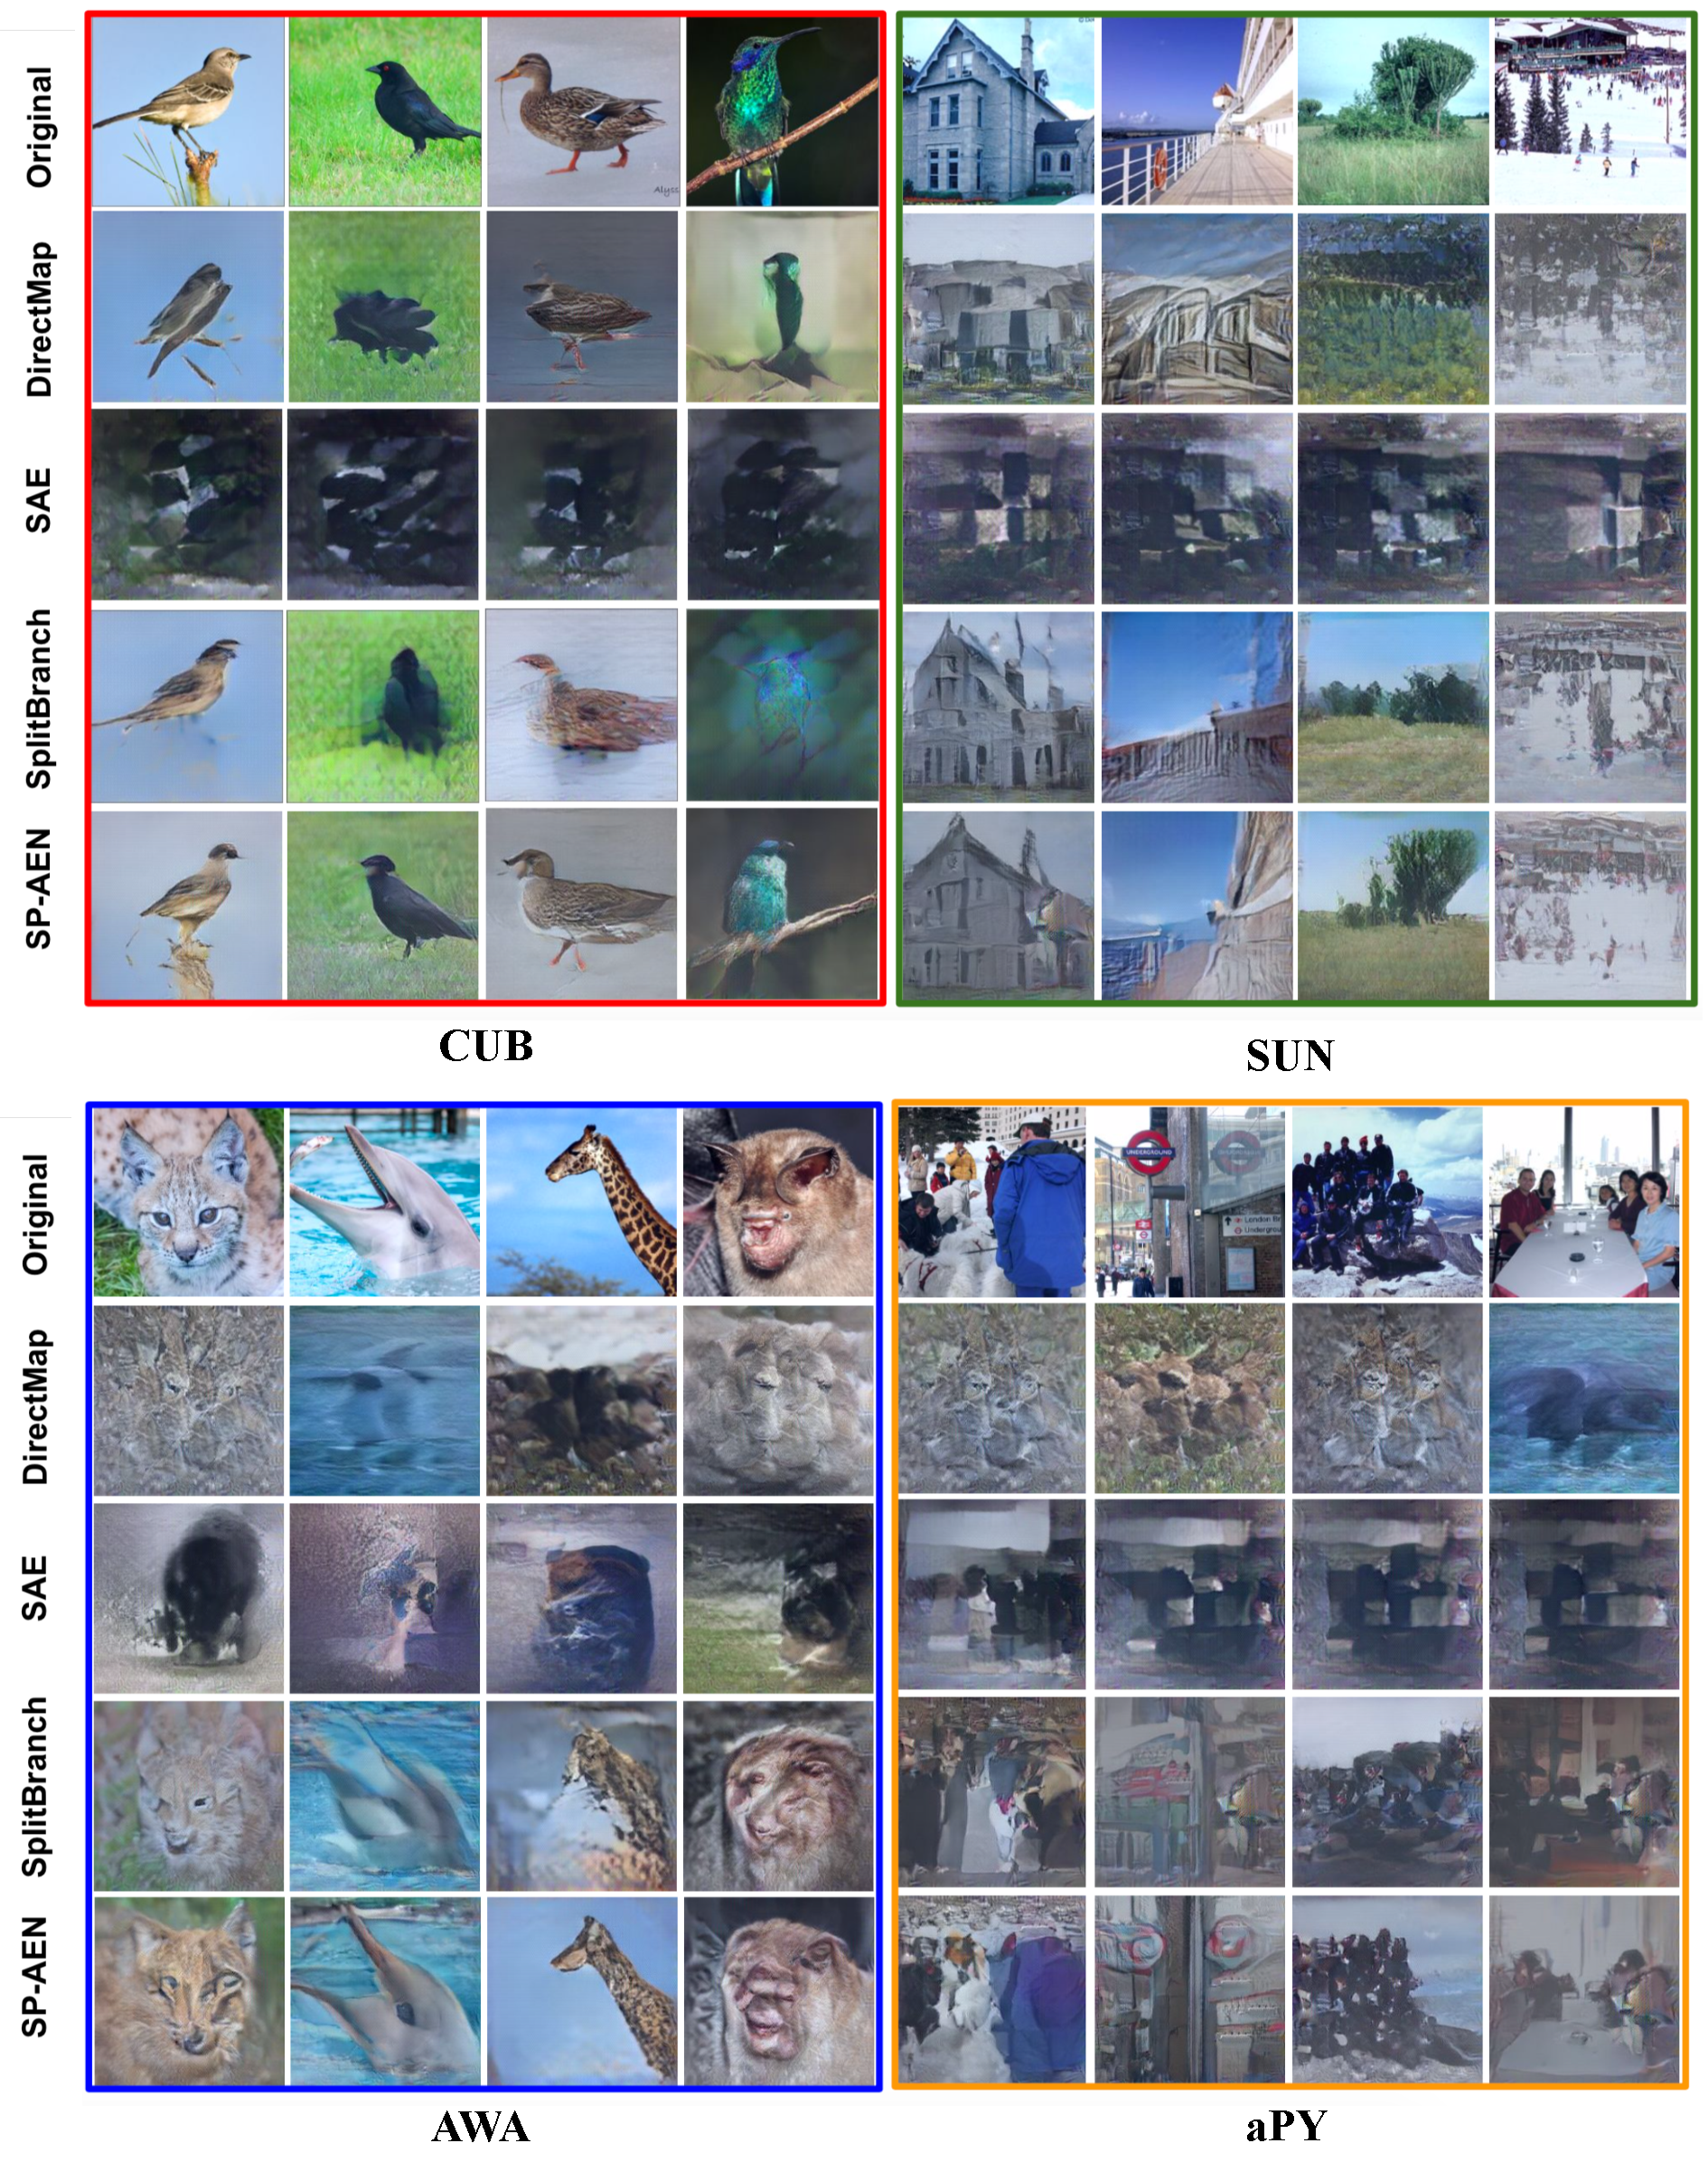
\includegraphics[width=\linewidth]{chapter3/res/conflict_visualization.pdf}
    \captionof{figure}{不同图像重建网络框架在数据集CUB、SUN、AWA、aPY上的重建结果。}
    \label{ch3:fig:conflict_visualization}
\end{figure}

图~\ref{ch3:fig:conflict_visualization}和表~\ref{ch3:tab:conflict_quantitative}分别表示四个数据集中测试集未见类别图像的重建图像和重建差异。




\section{本章小结}